\pdfminorversion 7
\pdfobjcompresslevel 3

\PassOptionsToPackage{table}{xcolor}
\documentclass[10pt,a4paper]{article}
%\documentclass[10pt,oneside,noprintercorrection]{article}
\special{papersize=210mm,297mm}


\usepackage[absolute]{textpos} 
\usepackage{pdfpages}
\usepackage[utf8]{inputenc}
\usepackage[T1]{fontenc}
\usepackage{cite}
\usepackage[francais]{babel}
\usepackage[bookmarks=false,colorlinks,linkcolor=blue]{hyperref}
\usepackage[top=4cm,bottom=3cm,left=3cm,right=3cm]{geometry}
\usepackage{graphicx}
\usepackage{wrapfig}
\usepackage{subfig}
\usepackage{eso-pic}
\usepackage{array}
\usepackage{listings}
\usepackage{color}
\usepackage[table]{xcolor}
\usepackage{url}
\usepackage{eurosym}
\usepackage{url}
\usepackage{textcomp}
\usepackage{fancyhdr} 
\usepackage{amsmath}
\usepackage{pict2e}
\usepackage{listings}
\usepackage{setspace}
\usepackage{float}
\usepackage[ruled,vlined,linesnumbered]{algorithm2e}
\usepackage[toc,page]{appendix} 
\usepackage{varwidth}
\onehalfspacing
\lstset{escapeinside={<@}{@>}}
\definecolor{lightgray}{gray}{0.9}


\title{Kmer signature in mitochondrial genomes for metagenome taxonomic assignation}

\author{Jérémy Fontaine and Samuel Blanquart}


\begin{document}
\maketitle

\section{Semaine 1: Mardi 1 Juillet}

\subsection{R\'eduction de la BDD}
~\\

La base de donnée complète totalise \textbf{30Go}, l'objectif était de réduire la taille de cette BDD en n'ayant les données qu'aux feuilles, pour les autres noeuds de l'arbre les données sont sous forme de lien symbolique. On obtient au final une BDD avec une taille de \textbf{1,1GO}.
~\\

Pour cela:
\\
\begin{itemize}
 \item Modification du fichier chemin-liste d’accession (voir figure \ref{resultatS})
  \item Script de remplissage des noeuds internes
\end{itemize}
~\\

\begin{figure}[H]
\begin{center}
\begin{tabular}{*{2}{c}}
  tax1/tax2/.../taxonFeuilleX : & accession\_1,...,accession\_N  \\
  tax1/tax2/.../taxonFeuilleY : & accession\_1,...,accession\_M  \\
\end{tabular}
\caption{\label{resultatS} Exemple de fichier "chemin: liste d'accession"}
\end{center}
\end{figure}
~\\

L'idée pour générer les liens symboliques est de faire remonter chaque données feuilles vers la racine de la BDD (figure \ref{linkage}).

\lstset{
	language=C,
	morecomment=[l][keywordstyle]{@\#},
	keywordstyle=\bfseries\ttfamily\color[rgb]{0,0,1},
	identifierstyle=\ttfamily,
	commentstyle=\color[rgb]{0.133,0.545,0.133},
	stringstyle=\ttfamily\color[rgb]{0.627,0.126,0.941},
	showstringspaces=false,
	basicstyle=\small,
	numberstyle=\footnotesize,
	numbers=left,
	stepnumber=1,
	numbersep=8pt,
	tabsize=2,
	breaklines=true,
	prebreak = \raisebox{0ex}[0ex][0ex]{\ensuremath{\hookleftarrow}},
	breakatwhitespace=false,
	aboveskip={1.5\baselineskip},
  columns=fixed,
  upquote=true,
  extendedchars=true,
  frame=single,
% backgroundcolor=\color{
}

\begin{figure}[H]
  

\begin{lstlisting}[numbers=left][caption=test]
      //
Pour chaque feuille l de la BBD
{
    /* On se deplace au niveau de la feuille */
    cd l;
    Pour chaque fichier f du dossier courant;
    {
      /* on se deplace dans la parent de cette feuille */  
      courant = pwd // commande unix
      tant que courant != racine
      {
        ln -s X
        /* on remonte d'un niveau */
        cd .. ;
        courant = pwd
      }
      /* on se replace a la feuille pour traiter le nouveau fichier */
      cd l;
    }
}                                            
\end{lstlisting}
\caption{\label{linkage} Algo lien symbolique}
\end{figure}
~\\

\subsection{Krona}
  krona est un utilitaire qui permet de visualiser des hiérarchies sous forme de camembert "zoomables". Pour cela cette hiérarchies doit être écrites sous formes de fichier xml. Krona construit ensuite un fichier html local, un navigateur web permet alors de visualiser le camembert. (figure \ref{krona})
  
  \begin{figure}[H]
\begin{lstlisting}[numbers=left][caption=test]
<node name="Alveolata">
    <genomes><val>1009</val></genomes>
    
    <node name="Apicomplexa">
        <genomes><val>993</val></genomes>
        ...
    </node>      
</node>                                          
\end{lstlisting}
\caption{\label{krona}Exemple simplifié d'un fichier pour krona}
\end{figure}
~\\

\subsection{Scripts dmp et krona}
  En fin de semaine, deux scripts ont été développés pour: 
  \begin{itemize}
    \item Récupérer/mettre à jour les fichiers dmp pour la construction de la bdd.
    \item Récupérer et installer krona
  \end{itemize}

\newpage
\section{Semaine 2: Lundi 7 Juillet}

\subsection{Générer le fichier weka à partir d'un dossier}
  L'idée première était de générer le fichier de comptage au format weka à partir d'un dossier. Pour se faire pour un dossier $D$ il faut effectuer le comptage pour ses sous dossier $d_1,...,d_n$ en prenant soins de récupérer chaque taxid pour chaque $d_i$ afin de lancer le programme de comptage {\textit{count\_kmer} avec les bons arguments. Le programme a était réalisé en Perl.\\ (trunk$/$generate\_learn$/$generate\_learn.pl)
  
  \subsubsection{Parallélisme}
  Au lieu de lancer le programme réalisé auparavant il est possible à partir des options d'utiliser plusieurs processeurs afin d'effectuer plusieurs comptage. Cependant même si le programme offre cette fonctionnalité lors de l'appel system de Perl pour appeler le programme C de comptage, Perl rend immédiatement la main et lance l'appel système suivant, le parallélisme se fait alors par défaut.
  
\subsection{Générer les fréquences de kmer aux feuilles}
  Le but de cette partie est de générer les fréquences uniquement aux feuilles. Ainsi pour construire le fichier weka à un noeud donnée $d$ il suffit d'aller récupérer les fréquences aux feuilles du sous arbre ayant pour pour racine $d$.  (trunk$/$generate\_learn$/$generate\_count.pl)
  

\newpage
\section{Semaine 3: Mardi 15 Juillet}
\subsection{Gestion d'erreur en C}
  Une partie de cette semaine a été consacrée au débogage du comptage écrit en C. En effet le comptage à la racine avec une fenêtre de 50, provoquait des erreurs 
  d'allocation mémoire. Ce problème fut régler grâce à la re-allocation de la mémoire. 
  \subsection{Taille du jeu de fréquences à la racine}
  Avec une taille de fenêtre glissante constante, la taille du fichier de fréquence est proportionnel à la somme des tailles de séquences (nombre de nucléotides totale). On a pu évaluer ainsi la taille du fichier de fréquence au plus haut niveau avec une fenêtre de taille 50 et le pattern \#\#\#\#. On obtiendrai au niveau de la racine, une taille de \textbf{123Go} pour le fichier de fréquence et un temps de \textbf{120 min}. Ainsi grâce aux graphes ci dessous on a pu évaluer le temps (fig. \ref{temps_cpt}) pour générer le fichier de fréquence et la taille de celui-ci (fig. \ref{taille_cpt}) sur l'ensemble des séquences (251 371 097 nucléotides).
  
  
\begin{figure}[H]
\begin{center}
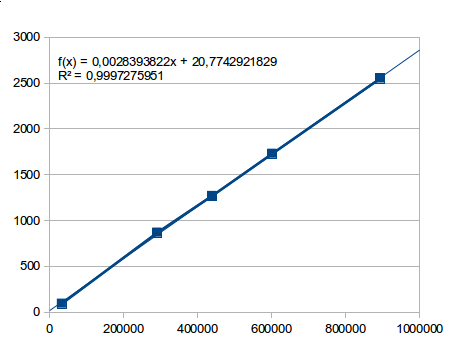
\includegraphics[scale=0.6]{./../img/graphe_temps.png}
\caption[Temps de du comptage]{\label{temps_cpt}Temps en seconde en fonction de la taille de la séquence avec une fenêtre de taille 50}
\end{center}
\end{figure}

\begin{figure}[H]
\begin{center}
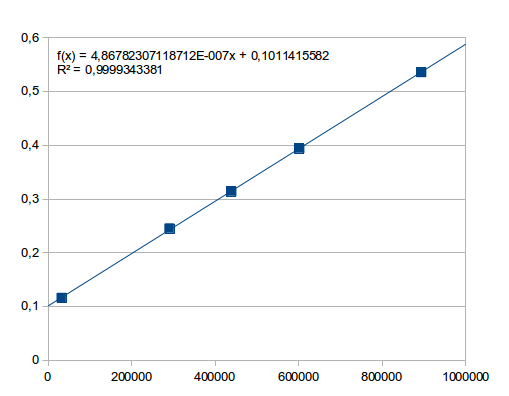
\includegraphics[scale=0.6]{./../img/graphe_taille.png}
\caption[Temps de du comptage]{\label{taille_cpt}Temps en seconde en fonction de la taille de la séquence avec une fenêtre de taille 50}
\end{center}
\end{figure}
  
\subsection{Passage aux objets}
Pour la suite du projet on décide de passer au c++ afin de tout gérer en tant qu'objet, on pourra ainsi plus aisément manipuler la table de fréquence en kmers. La génération
de données pour weka, la validation croisée...
\subsubsection{Les classes}
Pour le moment on ne manipule que trois classes:
\begin{itemize}
 \item classData: pour gérer les données (séquences,taille, nombre de jeux de données, responsable du comptage)
  \item classPattern: gestion d'un kmer
  \item FreqKmer: classe principale gérant principalement le tableau de fréquence.
\end{itemize}
~\\

L'objet à la possibilité de s'instancier à partir 
\begin{itemize}
 \item[.] D'un fichier fasta
 \item[.] D'un fichier contenant une liste de chemins vers des fichiers fasta.
\end{itemize}
~\\

De ce fait lorsqu'on souhaite obtenir la fréquence à un niveau, c'est au niveau des feuilles du sous arbre définit par ce niveau où l'on va effectuer le comptage.

En fin de semaine des tests de validation ont été rajoutés au programme. 


\newpage
\section{Semaine 4: Lundi 21 Juillet}
\subsection{Nouvelle manière de compter}
Suite à la réunion du 18 Juillet, on a décide de ne plus compter avec une fenêtre glissante. En effet cette façon générer des redondances dans la matrice de fréquences en kmers. Pour 
cela l'utilisateur à le choix de fournir son propre décalage (en nucléotide) sinon le programme utilise un décalage égale à 20\% de la taille de la fenêtre.

\subsection{Optimisation}
Dans un premier temps le programme à été revu pour prendre en compte ce décalage mais sans optimisation. L'optimisation consisterais à ne compter que les nouveau kmers lors du décalage de la fenêtre. Cette astuce était utilisée dans la version précédente. Mais étant que le décalage était égale à 1 nucléotides, une variable était suffisante pour mémoriser le kmer qui "sortait" de la nouvelle fenêtre comparé à la fenêtre précédente. On copiait ainsi la ligne de fréquence de la fenêtre précédente, on décrémenter la fréquence du kmer qui "sortait" et on calculait le nouveau kmer qui "entrait".
\\

Avec un décalage égale à $n$, on a $n$ kmer qui "sort" et $n$ nouveaux kmer à compter (entrant). Pour se faire on se propose d'utiliser deux tampons: 
\begin{itemize}
 \item[.] $courant$: correspondant à la ligne de comptage actuel, pour une fenêtre donnée.
 \item[.] $precedent$: correspondant à la ligne de comptage pour la fenêtre précédente.
\end{itemize}
~\\

Ces tampons ont la même taille que le nombre de kmer présent dans la fenêtre, soit si $f-k+1$ si $f$ est la taille de la fenêtre et $k$ la taille du kmer. Ainsi lors qu'on compte une toute première fois cela permet d'initialiser le tampon courant et de mémoriser tous les kmers rencontrés. Lorsqu'on passe à la fenêtre suivante si on effectue un décalage de $d$ nucléotides, il suffit donc:
\begin{itemize}
 \item[.] D'intervertir les deux tampons
 \item[.] De copier les bonnes parties dans le nouveau tampon, courant
 \item[.] Calculer les nouveaux kmers entrant et sauvegarder dans le tampon courant.
\end{itemize}
~\\

On obtient donc les kmers rencontrés, et on augmente dans le tableau de fréquence par rapport au tampon courant. Voir figure \ref{decalage} pour illustration, avec un kmer=\#\#\# et une fenêtre de taille 7.

\begin{figure}[H]
\begin{center}
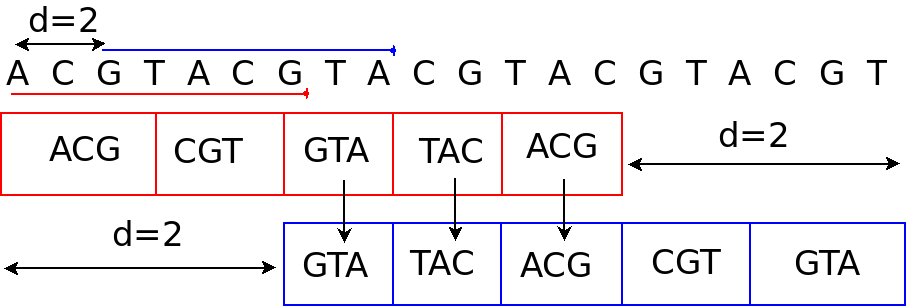
\includegraphics[scale=0.4]{./../img/decalage.png}
\caption[Principe du décalage]{\label{decalage}Principe du décalage avec une fenêtre de taille 7 et un tri-mers}
\end{center}
\end{figure}
~\\

Même si les tests sont ok et les tableaux de fréquences corrects. Il y a des cas où valgrind détecte des erreurs au niveau des ces buffers. D'autre erreurs par ailleurs sont également détecté par valgrind. L'objectif principal avant de continuer et d'éliminer toutes ces erreurs afin de continuer sur un programme "propre".


\newpage
\section{Semaine 5: Lundi 28 Juillet}
\subsection{Débogage}

Au fil de l'implémentation , des erreurs d'accès mémoire se sont accumulés. Ce fut une tâche longue de trouver toutes les sources d'erreur. A présent au fil du développement avant de passer une étape, valgrind et les tests doivent le programme. 

\subsection{Les cartes du tableau fréquences}

\subsubsection{D'une ligne à son jeu de donné, sa séquence}
Les semaines précédentes une carte a été mise en place, pour obtenir à partir d'une séquence d'un jeu de donnée l'indice de la ligne correspondante dans la table des fréquences.
Il a été jugé utile également d'avoir la carte inverse permettant à partir d'une ligne de retrouvé la séquence et le jeu de donnée associé. Cependant ces cartes sont insuffisantes ce qui est réellement important c'est de savoir pour une ligne à quelle taxon correspond la fréquence. La carte a donc été enrichie avec en amont le taxon associé par exemple avec la structure en figure \ref{struct}:

  

\begin{figure}[H]
\centering
\begin{varwidth}{\linewidth}
\begin{verbatim}
+taxon_alpha
|
|___+others
|   |__genomes.fasta (3 seqs)
|   
|___+taxon__A
|   |__genomes1.fasta (3 seqs)
|   |__genomes2.fasta (1 seqs)
|   |__genomes3.fasta (3 seqs)
|   |__genomes4.fasta (2 seqs)
|   
|___+taxon__B
|   |__genomes1.fasta (7 seqs)
|   
|___+taxon__C
|   |__genomes1.fasta (4 seqs)
|   |__genomes2.fasta (1 seqs)
|

\end{verbatim}
\end{varwidth}
\caption[Structure au niveau du taxon alpha]{\label{struct}Exemple de structure de l'arborescence au niveau du taxon alpha}
\end{figure}

Avec la structure donnée en figure \ref{struct} la carte associé serait celle présentée en figure \ref{map}.

\begin{figure}[H]
\begin{center}
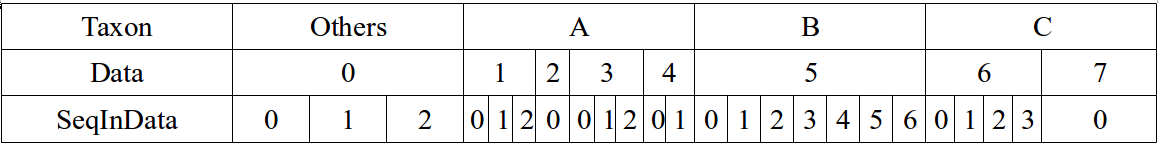
\includegraphics[scale=0.34]{./../img/map.png}
\caption{\label{map} Map dans le cas de la structure donnée en figure \ref{struct}, avec comme racine taxon\_\_alpha}
\end{center}
\end{figure}
~\\

Il est possible à présent,  à partir d'une ligne, de savoir à quelle séquence de quel jeu de données et surtout à quel taxon correspond la ligne de fréquence. C'est un bon point pour plus tard dans le développement des outils, en particulier pour l'écriture du fichier d’apprentissage puisque le taxid d'un taxon pour une ligne de fréquence donnée est connu. 
\\


Lors du test du programme sur une autre machine, il y a eu des erreurs avec les tests 15 à 18. Ceci est dû fait que lors de la lecture des sous dossier par l'appel système readdir, c++ ne garantie pas d'ordre. Un trie est alors effectue sur les chemins. C'est une étape qui permet au bon déroulement des tests 15 à 18 sur n'importe quel machine. Cependant il est possible de se passer du trie, dans ce cas le tableau de fréquence sera dans un ordre différent mais avec les cartes cela ne pose pas de soucis. 


\newpage
\section{Semaine 6: Lundi 04 Août}
\subsection{Échantillonnage}

L'objectif de cette semaine est de pouvoir échantillonner les données. C'est primordial pour la suite puisque comme nous l'avons vu 
à la figure \ref{taille_cpt} la taille du fichier de fréquence peut atteindre plus de 120Go, une taille trop importante pour l'outil d'apprentissage
\em {Weka}\em.

\subsubsection{Principe d'échantillonnage}

Pour échantillonner les données à un niveau taxonomique $alpha$, on se propose de considérer $SZ$ ($S$ample $S$ize) séquences tirées aléatoirement pour chaque sous taxon
de $alpha$.
\\

Si on reprend l'exemple de la figure \ref{struct} avec $SZ=5$, on a par exemple suite à un tirage aléatoire sans remise des séquences:

\begin{figure}[H]
\centering
\begin{varwidth}{\linewidth}
\begin{verbatim}
+taxon_alpha
|
|___+others
|   |__genomes.fasta (3 seqs)
|   
|___+taxon__A
|   |__genomes1.fasta (2 seqs)
|   |__genomes3.fasta (1 seqs) 
|   |__genomes4.fasta (2 seqs)
|   
|___+taxon__B
|   |__genomes1.fasta (5 seqs)
|   
|___+taxon__C 
|   |__genomes1.fasta (4 seqs)
|   |__genomes2.fasta (1 seqs)
|

\end{verbatim}
\end{varwidth}
\caption[Structure au niveau du taxon alpha après échantillonnage]{\label{struct_sample}Exemple de structure de l'arborescence au niveau du taxon alpha après l'échantillonnage pour $SZ=5$}
\end{figure}

\subsubsection{Méthode d'échantillonnage}

Pour échantillonner les données on va enrichir notre objet $FreqKmer$ par l'ajout d'un tableau de booléens à deux dimensions  pour savoir quelles séquences seront considérées dans le comptage de kmers.

\begin{figure}[H]
  

\begin{lstlisting}[numbers=left][caption=test]

/* Pour chaque sous taxon */
for(int i=0;i<nbChildTaxa;i++)
{
		nbSeqTaxa = getNSeqInTaxa(i);
		
		/* si on doit tirer plus de qu'il y a de seq alors on tire tout */
	  if(sampleSize>=nbSeqTaxa)
	  {
		  d = obtainStartLineTaxaInFastaList(i); /* indice debut data pour taxon courant i */
		  f = obtainEndLineTaxaInFastaList(i); /* indice fin data pour taxon courant i */
      
      /* Pour chaque data du taxon courant */
      for(int j=d; j<=f;j++)
		  {
		     /* Pour chaque sequence */
	      for(int k=0;k<data[j]->getNtaxa();k++)
			  {
			    /* On prend la k-eme sequence du j-eme data */
				  mask_tmp[j][k]=true;
			  }
		  }
	  }
	  else
	  {
	    	/* on tire sampleSize parmi les nbSeqTaxa sequences
			 * dans le taxon courant
			 * (tirage sans remise pour les seq.!)
			 */
			randomTab(&candidates,nbSeqTaxa,sampleSize);
			/* je mets a jour mon mask selon les candidats trouves */
			maskTab(&candidates,mask_tmp,i);
	  }
                       
\end{lstlisting}
\caption{\label{sampleMe} Algo d'échantillonnage}
\end{figure}
~\\


\begin{figure}[H]
  

\begin{lstlisting}[numbers=left][caption=test]

/* tirage sans remise de sampleSize sequences 
parmi tabSize sequences */
void randomTab(vector<int> *result,int tabSize,int sampleSize)
{
  
	int *tmp = new int[tabSize];
	int r = -1;
	
	/* Borne du tirage au depart on peut tirer toutes les sequences */
	int sup = tabSize;
	int val_tmp;

  /* on cree un tableau contenant 
   * initialement les indices, on va ainsi tirer les indices des 
   * sequences a considerer pour l'echantillon */
	for(int i=0;i<tabSize;i++)
	{
		tmp[i]=i;
	}

  /* On tire sampleSize indice */
	for(int j=0;j<sampleSize;j++)
	{

		r = rand() % sup;
		/* on met la valeur tiree a la fin du tableau 
		 * et on n'y touche plus */
		val_tmp = tmp[sup-1];
		
		/* on met l'indice dans le resultat */
		result->push_back(tmp[r]);
		tmp[sup-1] = tmp[r];
		tmp[r] = val_tmp;
    
    /* la borne du tirage diminue */
		sup--;

	}

}
               
\end{lstlisting}
\caption{\label{tirage} Algo de tirage sans remise}
\end{figure}
~\\


\newpage
\section{Semaine 7: Lundi 11 Août}
L'objectif de cette semaine est de pouvoir générer un jeu de données pour la validation croisée sous weka.

\subsection{Classer les données}

Avant de poursuivre, la base de donnée à été modifiée afin des données classée. Ceci permet de mieux se retrouver entre séquences d'acides aminées, nucléotidiques, fichier genbank, les enzymes (cox1,cox2...) ...

~\\
Chaque dossier comporte en plus des dossiers des sous taxons:

\begin{itemize}
 \item[.]Un dossier \textit{frequencies} où sera rangées les fréquences de kmers
  \item[.]un dossier \textit{data} correspondant aux données génétiques et étant constitué
  \begin{itemize}
 \item Un dossier \textit{fasta} où sera rangées les séquences, constitué de deux sous dossiers 
  \begin{itemize}
 \item[*]\textit{aminoAcids} contenant les séquences d'acides aminés, chaque cox, cytb,...sont également rangé dans un dossier de même nom. 
 
  \item[*]\textit{nucletotides} contenant les séquences nucléotidiques, de même ici chaque cox, cytb,...sont également rangé dans un dossier de même nom. Ce dossier contient en plus un dossier \textit{genomes} contenant tous le génome complet (voir figure \ref{dossierCox}).
  
\end{itemize}
  \item un dossier \textit{genbank} contenant les fichiers genbank associés au taxon courant
  
\end{itemize}
\end{itemize}
~\\

\begin{figure}[H]
\begin{center}
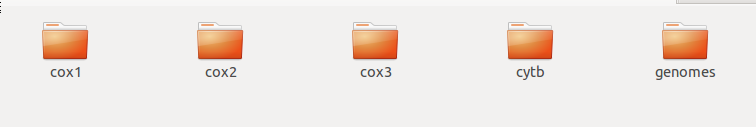
\includegraphics[scale=0.5]{./../img/dossier.png}
\caption{\label{dossierCox} Dossiers lorsqu'on se trouve dans le dossier data/fasta/nucleotides d'un taxon.}
\end{center}
\end{figure}
~\\

Cette façon de classer les données permet à l'utilisateur de pouvoir spécifier sur quelles séquences il souhaites travailler en indiquant les mots clés \textit{cox1},\textit{cox2},...ou \textit{genomes}.

\subsection{Validation croisée}

Le principe de la validation croisée, est de produire deux fichiers pour weka:
\begin{itemize}
  \item[.] Un pour l'apprentissage (80\% des séquences)
  \item[.] et un autre pour la prédiction (20\% des séquences)
\end{itemize}

Les deux fichiers de fréquences doivent avoir été construits à partir de séquences distinctes. Par exemple si $D$ est l'ensemble de nos séquences alors
on doit construire le fichier d'apprentissage à partir d'un sous ensemble $A$ et le fichier de prédiction à partir d'un sous ensemble $P$ de 
tel sorte que $A \cup P = D $ et  $ A \cap P = \emptyset $  

\subsection{Classification sous java}

Afin de pouvoir charger les données on est forcé d'utiliser le classifieur Bayes car c'est le seul à ce jour, 
permettant de charger les données petit à petit. 

\subsubsection{Quelques résultats}
On obtient avec le programme implémenté en java et donc avec le classifieur de Bayes 90\% d'instances correctement classées, alors qu'avec LibSVM on obtenait plus de 98\%. 


{\scriptsize \textit{Implémenter nous même notre LibSVM ?...}}


\newpage
\section{Semaine 7: Lundi 18 Août}



\newpage
\section{Semaine 8: Lundi 25 Août}


%commentaire

\end{document}



